\documentclass[12pt,a4]{article}
\usepackage[english]{babel}
\usepackage[utf8]{inputenc}
\usepackage[T1]{fontenc}
\usepackage{geometry}
\usepackage{float}
\geometry{
	a4paper,
	left=20mm,
	right=20mm,
	top=20mm,
	bottom=20mm,
}
% Useful packages
\usepackage{amsmath}
\usepackage{bm}
\usepackage{graphicx}
\usepackage[colorlinks=true, allcolors=blue]{hyperref}
\usepackage[framed,numbered,autolinebreaks,useliterate]{mcode} % MATLAB style code


\begin{document}
\section{Constants and Dimensions}

\begin{table}[H]
	\centering
	\begin{tabular}{l|lcl}
		Symbol       & Value                           & Unit             & Description                                       \\\hline
		$g$          & $9.81$                          & $\frac{m}{s^2}$  & acceleration of gravity                           \\
		$\rho$       & $1025$                          & $\frac{kg}{m^3}$ & density of water                                  \\
		$L$          & $ 2.0 $                         & $m$              & length of hull                                    \\
		$B$          & $ 1.08 $                        & $m$              & beam of hull                                      \\
		$m$          & $ 55.0 $                        & $ kg $           & mass of hull                                      \\\hline
		$r_g^{hull}$ & $ \begin{bmatrix}0.2&0&-0.2\end{bmatrix}^T $ & $ m$             & CG of hull                                        \\
		$R_{44} $    & $0.4 \cdot B$                   & $m$              & radius of gyration                                \\
		$R_{55} $    & $0.25\cdot L$                   & $m$              & radius of gyration                                \\
		$R_{66} $    & $0.25\cdot L$                   & $m$              & radius of gyration                                \\
		$T_{yaw}$    & $ 1$                            & $s $             & time constant in yaw                              \\
		$U_{max}$    & $ 6 $                           & $ knot $         & max forward speed                                 \\\hline
		$B_{pont} $  & $0.25 $                         & $ m $            & beam of one pontoon                               \\
		$y_{pont} $  & $0.395$                         & $ m $            & distance from centerline to waterline area center \\
		$Cw_{pont}$  & $0.75 $                         & $ - $            & waterline area coefficient                        \\
		$Cb_{pont}$  & $0.4$                           & $ - $            & block coefficient                                 \\
		$ $          & $ $                             & $  $             &                                                   \\
	\end{tabular}
\end{table}

Waterline area of one pontoon
\begin{equation}
	Aw_{pont} = Cw_{pont} L B_{pont}
\end{equation}

\section{Skew symetric matrix}

\begin{equation}
	S\left(\begin{bmatrix}a_1\\a_2\\a_3\end{bmatrix}\right) =
	\begin{bmatrix}
		0    & -a_3 & a_2  \\
		a_3  & 0    & -a_1 \\
		-a_2 & a_1  & 0
	\end{bmatrix}
\end{equation}


\section{Kinetics}
\begin{align}
	\nu_1 & = \begin{bmatrix}u & v & w\end{bmatrix}^T & \nu_2 & = \begin{bmatrix}p & q & r\end{bmatrix}^T
\end{align}
Inertia matrix of hull in CG
\begin{equation}
	I_g^{CG} = m \cdot \text{diag}\begin{bmatrix}R_{44}^2, R_{55}^2, R_{66}^2\end{bmatrix}
\end{equation}
CG location corrected for payload
\begin{equation}
	r_g = \frac{m \cdot r_g^{hull} + m_p \cdot r_p}{m+mp}
\end{equation}
Inertia matrix of hull and payload in CO
\begin{equation}
	I_g = I_g^{CG} - m \cdot S(r_g)^2 - m_p \cdot S(r_p)^2
\end{equation}




\begin{align}
	M_{RB}^{CG}                & =
	\begin{bmatrix}
		(m+m_p)I & 0   \\
		0        & I_g
	\end{bmatrix} &
	C_{RB}^{CG}(\nu_2)         & =
	\begin{bmatrix}
		(m+m_p) S(\nu_2) & 0             \\
		0                & -S(I_g \nu_2)
	\end{bmatrix}
\end{align}



Transform $M_{RB}$ and $C_{RB}$ from the $C_G$ to the $C_O$
\begin{equation}
	H = \begin{bmatrix} I & S(r_g)^T\\ 0  & I \end{bmatrix}
\end{equation}

\begin{align}
	M_{RB}        & = H^T M_{RB}^{CG} H        \\
	C_{RB}(\nu_2) & = H^T C_{RB}^{CG}(\nu_2) H \\
\end{align}

\section{Relative velocity}
Water current surge and sway velocity
\begin{align}
	u_c & = v_{cur} \cos(\beta_{cur} - \psi) \\
	v_c & = v_{cur} \sin(\beta_{cur} - \psi)
\end{align}
Where $v_{cur}$ is the current velocity, $\beta_{cur}$ is the current direction in \textit{rad} and $\psi$ is the yaw of the vessel.
Relative velocity vector
\begin{equation}
	\nu_r = \nu - \begin{bmatrix}u_c & v_c & 0 & 0 & 0 & 0\end{bmatrix}^T
\end{equation}
In the case of no current we have
\begin{equation}
	\nu_r = \nu
\end{equation}
\section{Hydrodynamics}
Hydrodynamic added mass

\begin{equation}
	M_A =
	\begin{bmatrix}
		mI & 0   \\
		0  & I_g
	\end{bmatrix}
	M_{A,coef}
\end{equation}

\begin{equation}
	M_{A,coef} = \text{diag}\left(\begin{bmatrix}0.1 & 1.5 & 1.0 & 0.2 & 0.8 & 1.7\end{bmatrix}\right)
\end{equation}


\begin{align}
	C_A(\nu_{r,1},\nu_{r,2}) & =
	\begin{bmatrix}
		0                                         & -S(M_{A,11}\nu_{r,1} + M_{A,12}\nu_{r,2}) \\
		-S(M_{A,11}\nu_{r,1} + M_{A,12}\nu_{r,2}) & -S(M_{A,21}\nu_{r,1} + M_{A,22}\nu_{r,2})
	\end{bmatrix}   \\
	                         & =
	\begin{bmatrix}
		0                        & -S(0.1 \cdot m\nu_{r,1}) \\
		-S(0.1 \cdot m\nu_{r,1}) & -S(1.5 \cdot m\nu_{r,2})
	\end{bmatrix}
\end{align}

System mass and Coriolis-centripetal matrices
\begin{align}
	M & = M_{RB} + M_A                             \\
	C & = C_{RB}(\nu_2) + C_A(\nu_{r,1},\nu_{r,2})
\end{align}


\section{Hydro statics}
Water volume displacement
\begin{equation}
	\nabla = \frac{m+m_p}{\rho}
\end{equation}
Draft
\begin{equation}
	T = \frac{\nabla}{2 Cb_{pont} B_{pont} L}     % draft
\end{equation}

\begin{equation}
	KB = \frac{1}{3}(5\frac{T}{2} - \frac{\nabla}{2 L B_{pont}});
\end{equation}

\begin{align}
	I_T & = \frac{2}{12} L B_{pont}^3 \frac{6\cdot Cw_{pont}^3}{(1+Cw_{pont})(1+2Cw_{pont})} + 2 \cdot Aw_{pont} y_{pont}^2 \\
	I_L & = \frac{0.8\cdot 2}{12}  B_{pont}  L^3
\end{align}

\begin{align}
	GM_T & = KB + \frac{I_T}{\nabla} - T + r_{g,z}  \\
	GM_L & = KB + \frac{I_L}{\nabla}  - T + r_{g,z} \\
\end{align}


\begin{equation}
	G_{CF} = \begin{bmatrix}
		0 & 0 & 0                       & 0                    & 0                   & 0 \\
		0 & 0 & 0                       & 0                    & 0                   & 0 \\
		0 & 0 & \rho  g  (2  Aw_{pont}) & 0                    & 0                   & 0 \\
		0 & 0 & 0                       & \rho  g \nabla  GM_T & 0                   & 0 \\
		0 & 0 & 0                       & 0                    & \rho  g \nabla GM_L & 0 \\
		0 & 0 & 0                       & 0                    & 0                   & 0
	\end{bmatrix}
\end{equation}



%LCF = -0.2;
%H = Hmtrx([LCF 0 0]);               % transform G_CF from the CF to the CO

\begin{equation}
	G = H^T  G_{CF}  H
\end{equation}

% Natural frequencies
\begin{align}
	\omega_3 & = \sqrt{G_{33}/M_{33}} \\
	\omega_4 & = \sqrt{G_{44}/M_{44}} \\
	\omega_5 & = \sqrt{G_{55}/M_{55}}
\end{align}

\section{Linear Damping}
\begin{equation}
	h(r) =
	\begin{bmatrix}
		-24.4 \frac{g}{U_{max}}             \\
		0                                   \\
		-2 \cdot 0.3 \cdot \omega_3  M_{33} \\
		-2 \cdot 0.2 \cdot \omega_4  M_{44} \\
		-2 \cdot 0.4 \cdot \omega_5  M_{55} \\
		\frac{-M_{66}}{T_{yaw}}
	\end{bmatrix} + \begin{bmatrix}0\\0\\0\\0\\0\\  \frac{-M_{66}}{T_{yaw}} 10 \cdot abs(r)\end{bmatrix}
\end{equation}
The matrix to the right includes non-linear dampimg for yaw

\begin{equation}
	\tau_{damp}(r) = h(r) \bullet \nu_r
\end{equation}

\section{Crossflow Drag}
The crossflow is computed using strip theory and is a function of $\nu_r$
\begin{equation}
	\tau_{cf} =
	\begin{bmatrix}0\\Yh\\0\\0\\0\\Nh\end{bmatrix}
\end{equation}
$\tau_{cf}$ Has components only in \textit{v} and \textit{r}

First-order fitting
\begin{equation*}
	\bm{\tau}_{cf} = \left[\begin{array}{c} 0\\ 1.2907e-16\,r-12.2363\,v-4.8735e-17\\ 0\\ 0\\ 0\\ -5.9740\,r-5.1780e-16\,v-3.6373e-19 \end{array}\right]
	\approx \left[\begin{array}{c} 0\\ -12.2363\,v\\ 0\\ 0\\ 0\\ -5.9740\,r \end{array}\right]
\end{equation*}
Second-order fitting
\begin{equation*}
	\bm{\tau}_{cf} = \left[\begin{array}{c} 0\\ 0.1824\,r-0.0666\,v-41.8276\,r\,\left|r\right|-1.6409\,r\,\left|v\right|-122.0516\,v\,\left|v\right|+0.0019\\ 0\\ 0\\ 0\\ 0.0535\,v-0.1471\,r-2.5043\,r\,\left|r\right|-88.3910\,r\,\left|v\right|-0.2423\,v\,\left|v\right|-0.0015 \end{array}\right]
\end{equation*}

\begin{figure}[H]
	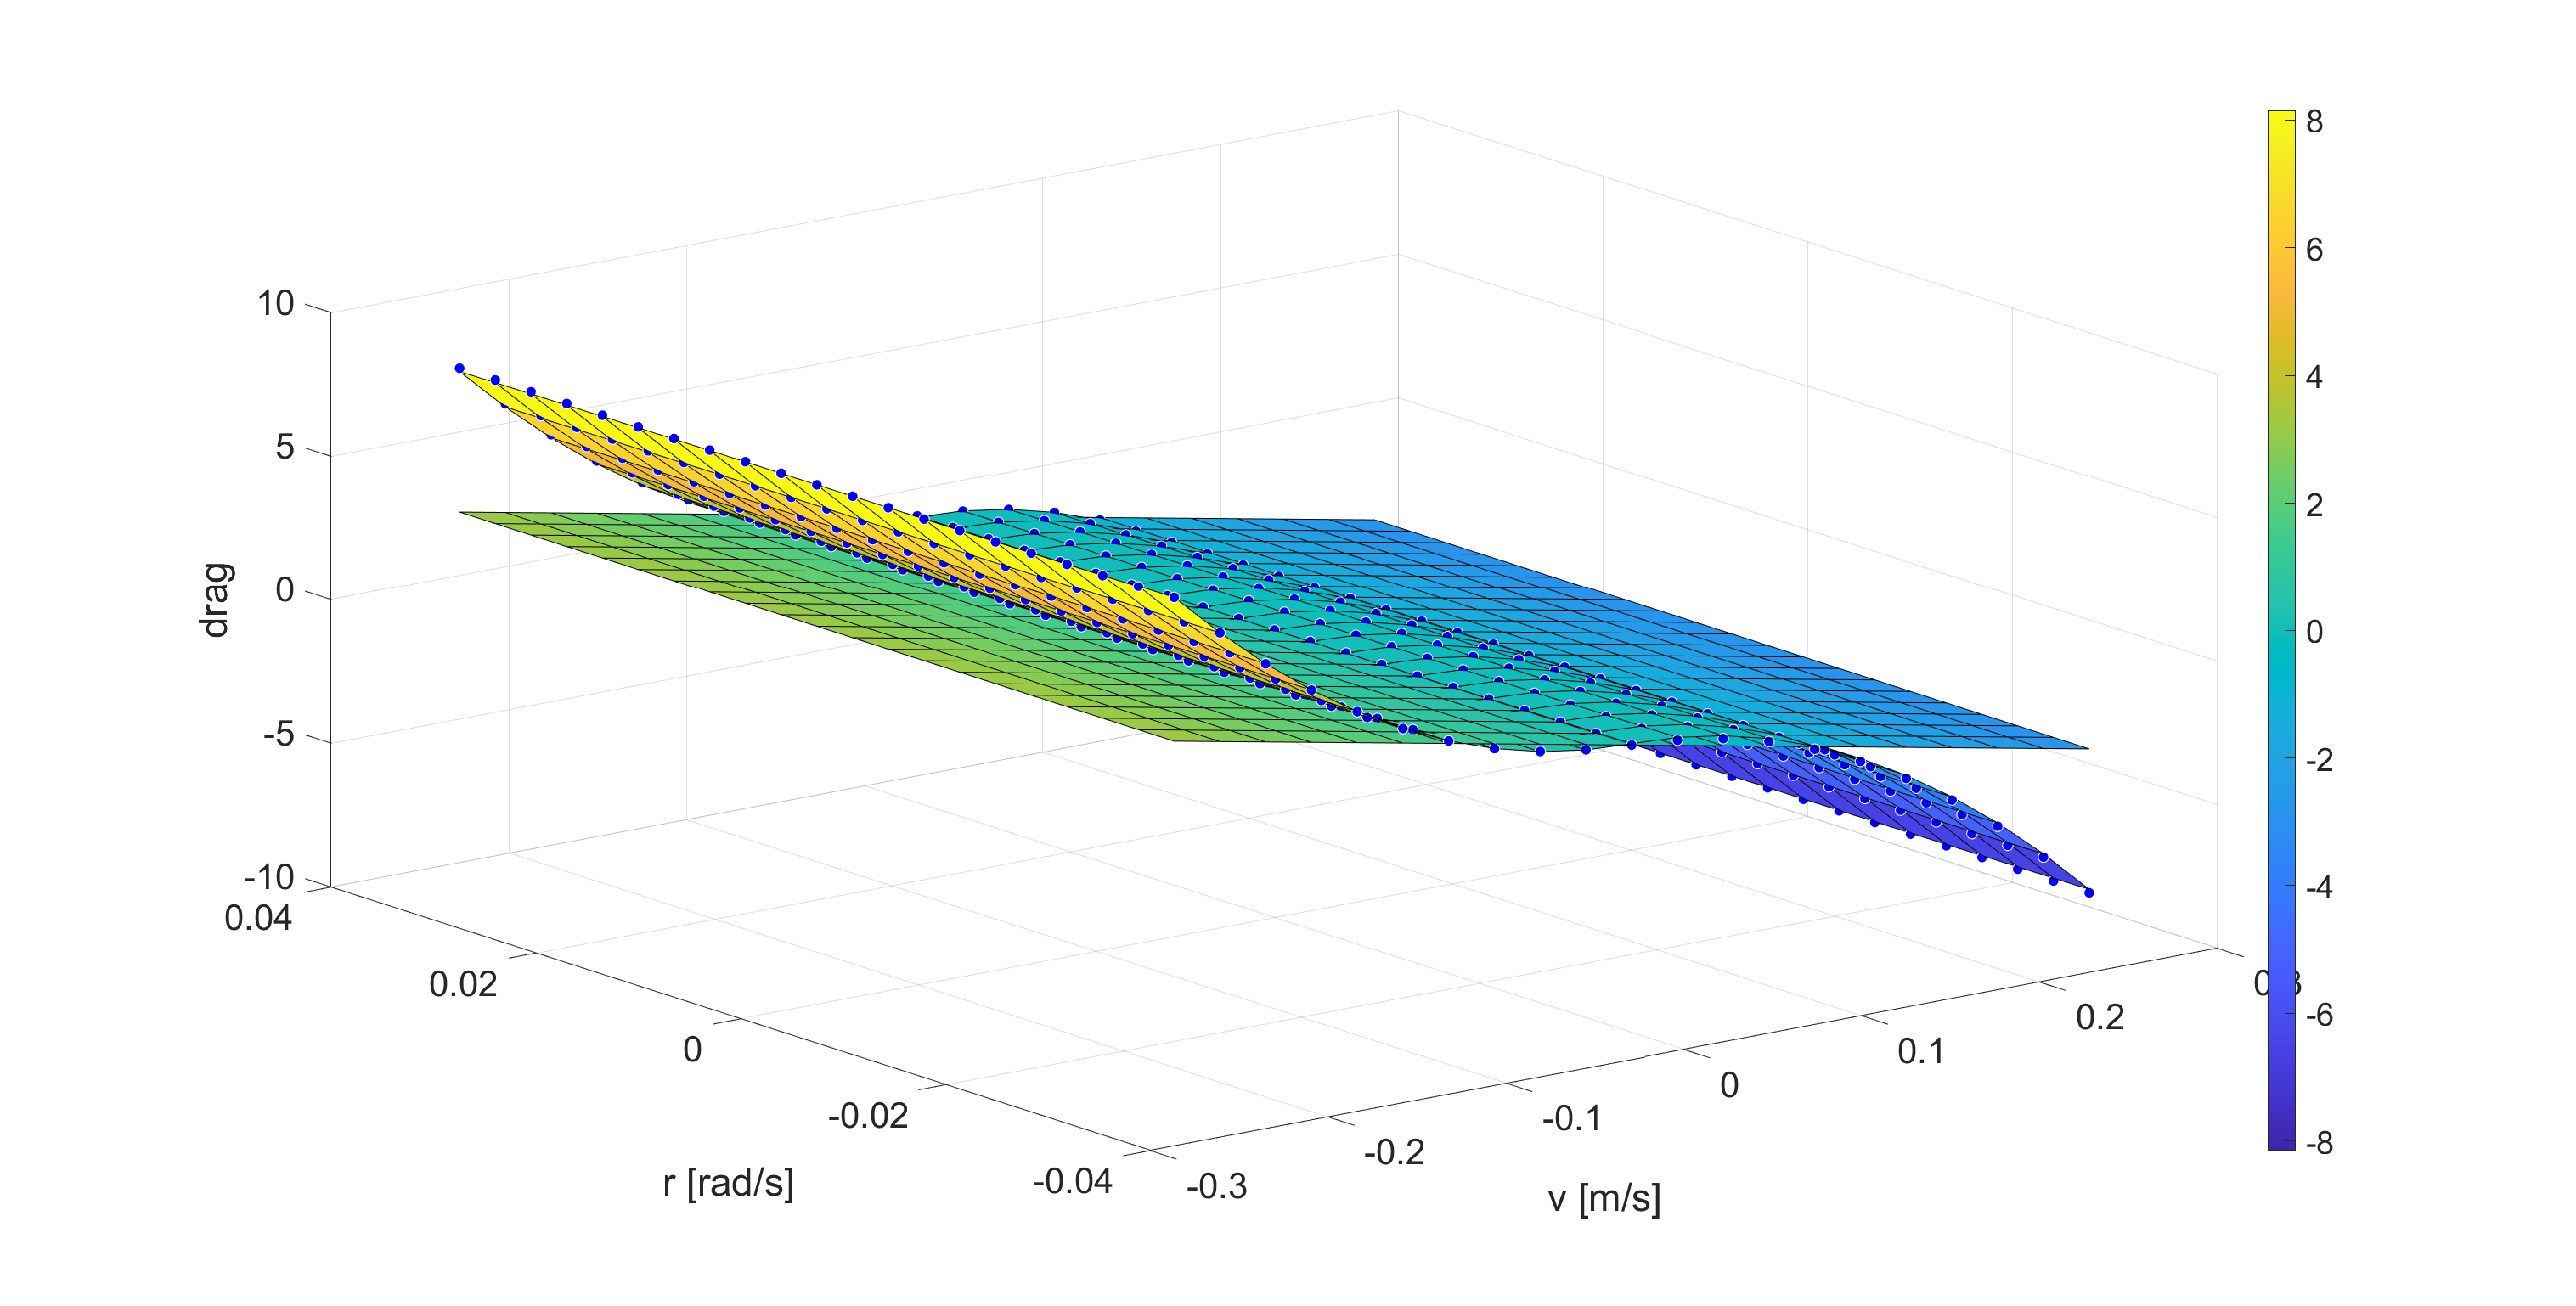
\includegraphics[width = \textwidth]{graphics/SwayDampingFitting.eps}
	\caption{Linearized crossflow damping in sway}
	\label{fig:SwayDampingFitting}
\end{figure}
\begin{figure}[H]
	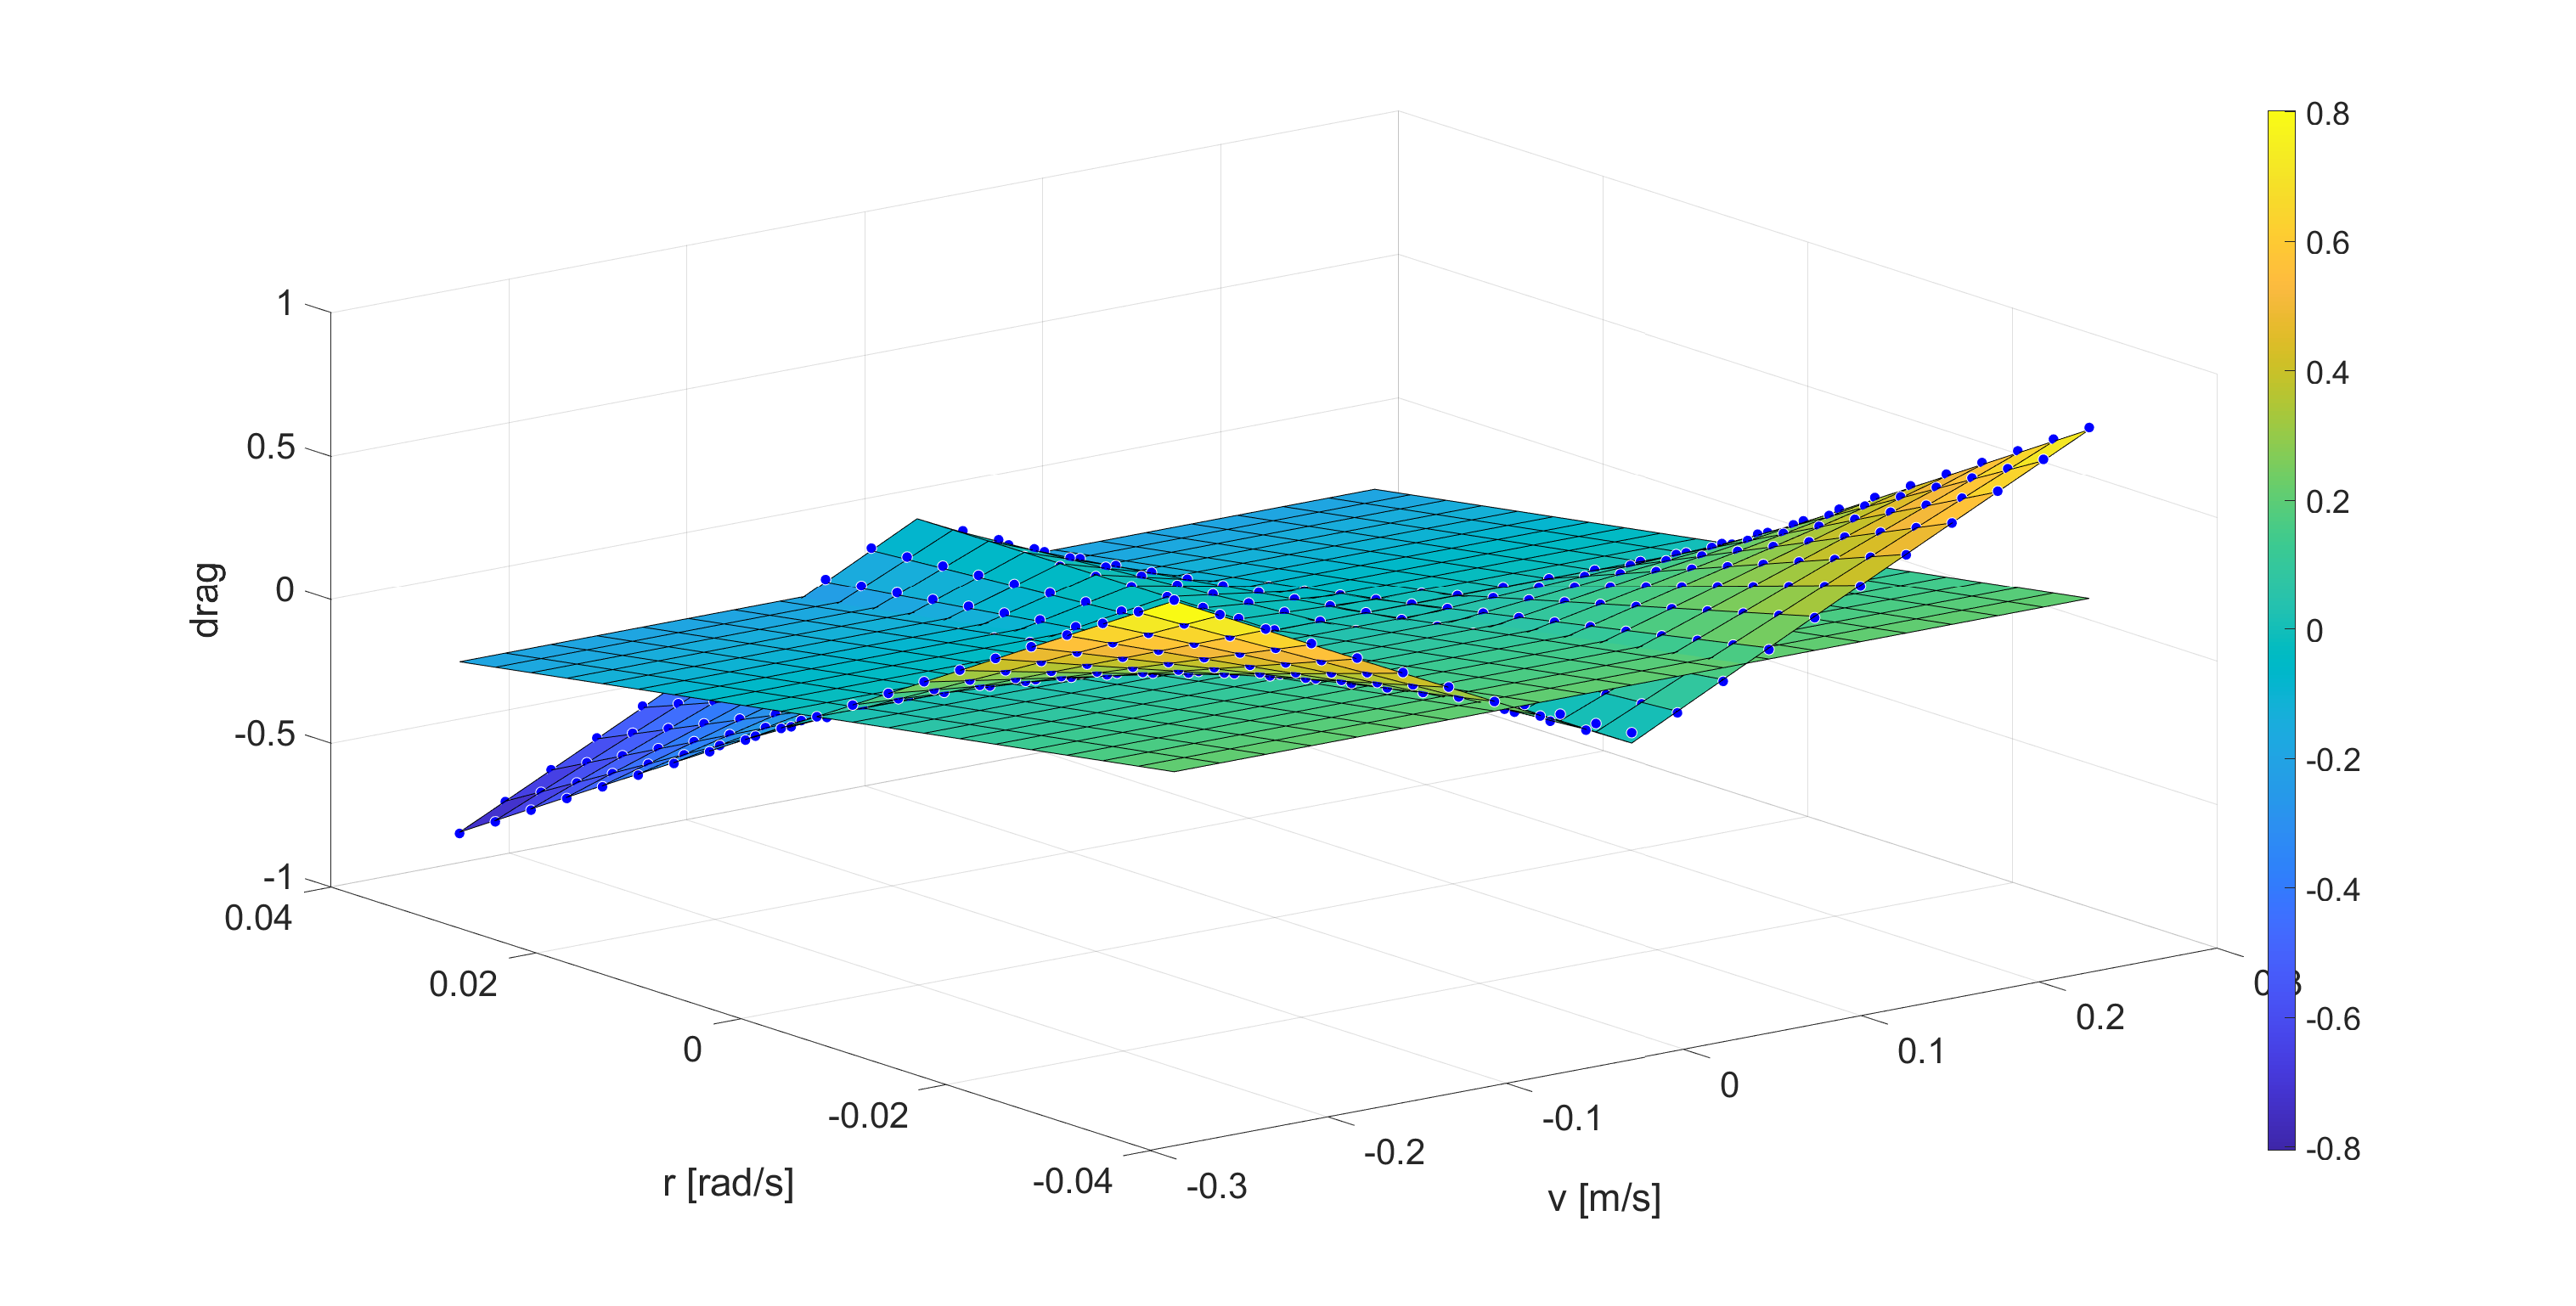
\includegraphics[width = \textwidth]{graphics/YawDampingFitting.eps}
	\caption{Linearized crossflow damping in yaw}
	\label{fig:YawDampingFitting}
\end{figure}

\section{Ballast}
\begin{lstlisting}[frame=single]
	trim_setpoint = 280;
	persistent trim_moment;
	if isempty(trim_moment)
	trim_moment = 0;
	end
	.
	.
	g_0 = [0 0 0 0 trim_moment 0]';
	.
	.
	trim_moment = trim_moment + 0.05 * (trim_setpoint - trim_moment);
\end{lstlisting}

\begin{equation}
	g_0 =
	\begin{bmatrix}0\\0\\0\\0\\trim\_moment\\0\end{bmatrix}
\end{equation}

$g_0$ represents a dynamic torque in \textit{q} (pitch)

\section{Transformation}
\begin{equation}
	R = R_z R_y R_x =
	\begin{bmatrix}
		\cos(\psi) & -\sin(\psi) & 0 \\
		\sin(\psi) & \cos(\psi)  & 0 \\
		0          & 0           & 1
	\end{bmatrix}
	\begin{bmatrix}
		\cos(\theta)  & 0 & \sin(\theta) \\
		0             & 1 & 0            \\
		-\sin(\theta) &   & \cos(\theta)
	\end{bmatrix}
	\begin{bmatrix}
		1 & 0          & 0           \\
		0 & \cos(\phi) & -\sin(\phi) \\
		0 & \sin(\phi) & \cos(\phi)
	\end{bmatrix}
\end{equation}

\begin{equation}
	T =
	\begin{bmatrix}
		1 & \sin(\phi)\tan(\theta)           & \cos(\phi)\tan(\theta)           \\
		0 & \cos(\phi)                       & -\sin(\phi)                      \\
		0 & \dfrac{\sin(\phi)}{\cos(\theta)} & \dfrac{\cos(\phi)}{\cos(\theta)}
	\end{bmatrix}
\end{equation}

\begin{equation}
	J = \begin{bmatrix}
		R & 0 \\
		0 & T
	\end{bmatrix}
\end{equation}

\section{State derivative}
\begin{align}
	M \dot{\nu} + C \nu_r + G \eta + g_0 & = \tau + \tau_{damp} + \tau_{cf} \\
	\dot{\eta}                           & = J(\eta)\nu
\end{align}

\begin{equation}
	\dot{x} =
	\begin{bmatrix}\dot{\nu}\\\dot{\eta}\end{bmatrix}
	=
	\begin{bmatrix}
		M^{-1}(\tau + \tau_{damp}(r) + \tau_{cf}(\nu_r) - C  \nu_r - G  \eta - g_0) \\
		J \nu
	\end{bmatrix}
\end{equation}


\begin{align*}
	M & = H^T M_{RB}^{CG} H + M_A \\
	  & =
	\begin{bmatrix} I & 0 \\ S(r_g)  & I \end{bmatrix}
	\begin{bmatrix}
		(m+m_p)I & 0   \\
		0        & I_g
	\end{bmatrix}
	\begin{bmatrix} I & S(r_g)^T\\ 0  & I \end{bmatrix}
	+
	\begin{bmatrix}
		mI & 0   \\
		0  & I_g
	\end{bmatrix}
	M_{A,coef}                    \\
	  & =
	(m+m_p)
	\begin{bmatrix}
		I      & S(r_g)^T            \\
		S(r_g) & S(r_g) I_g S(r_g)^T
	\end{bmatrix}
	+
	\begin{bmatrix}
		mI & 0   \\
		0  & I_g
	\end{bmatrix}
	M_{A,coef}
\end{align*}

\begin{align*}
	C & = H^T C_{RB}^{CG}(\nu_2) H  + C_A(\nu_{r,1},\nu_{r,2}) \\
	  & =
	\begin{bmatrix} I & 0 \\ S(r_g)  & I \end{bmatrix}
	\begin{bmatrix}
		(m+m_p) S(\nu_2) & 0             \\
		0                & -S(I_g \nu_2)
	\end{bmatrix}
	\begin{bmatrix} I & S(r_g)^T\\ 0  & I \end{bmatrix}
	+
	\begin{bmatrix}
		0                        & -S(0.1 \cdot m\nu_{r,1}) \\
		-S(0.1 \cdot m\nu_{r,1}) & -S(1.5 \cdot m\nu_{r,2})
	\end{bmatrix}                                 \\
	  & =
	(m+m_p)
	\begin{bmatrix}
		S(\nu_2)        & S(\nu_2)  S(r_g)^T          \\
		S(r_g) S(\nu_2) & -S(r_g)S(I_g \nu_2)S(r_g)^T
	\end{bmatrix}
	+
	\begin{bmatrix}
		0                        & -S(0.1 \cdot m\nu_{r,1}) \\
		-S(0.1 \cdot m\nu_{r,1}) & -S(1.5 \cdot m\nu_{r,2})
	\end{bmatrix}
\end{align*}


\section{All system equations}
The equations can be found in \textbf{AutoDocking/Models/Primitive/SysEq6DOF.mat}
\begin{multline}
	\dot{u} = 0.0054\,\tau _{q}-1.3169\,q+0.0175\,\tau _{u}+5.3523e-04\,\tau _{w}-16.0798\,\theta \\-1.3574\,u-0.2925\,w-12.1092\,z+0.3371\,p\,r-0.0147\,p\,v-0.0265\,q\,u-1.8664\,q\,w\\+2.3477\,r\,v+0.2649\,u\,w+0.0177\,p^2+0.1866\,q^2+0.1690\,r^2
\end{multline}
\begin{multline}
	\dot{v} = 0.2504\,p+4.9601\,\phi +0.0629\,r-0.0046\,\tau _{p}-0.0014\,\tau _{r}+0.0078\,\tau _{v}\\-7.8984e-04\,v-0.0364\,p\,q+0.1167\,q\,r+0.7867\,p\,w-0.4028\,r\,u-0.1266\,v\,w+0.3215\,r\,\left|r\right|\\+0.1389\,r\,\left|v\right|-0.9472\,v\,\left|v\right|+4.4851e-05
\end{multline}
\begin{multline}
	\dot{w} = 0.0029\,\tau _{q}-0.7243\,q+5.3523e-04\,\tau _{u}+0.0094\,\tau _{w}-22.5556\,\theta \\-0.0415\,u-5.1289\,w-75.2186\,z-0.0146\,p\,r-1.2581\,p\,v+0.5354\,q\,u-0.0265\,q\,w\\+0.0412\,r\,v+0.1457\,u\,w-0.0903\,p^2-0.0974\,q^2-0.0071\,r^2
\end{multline}
\begin{multline}
	\dot{p} = 0.2272\,r-67.3414\,\phi -3.3993\,p+0.0625\,\tau _{p}-0.0050\,\tau _{r}-0.0046\,\tau _{v}\\+0.0010\,v-0.1257\,p\,q-0.5847\,q\,r+0.1266\,p\,w-0.3545\,r\,u+1.7190\,v\,w+2.4254\,r\,\left|r\right|\\+0.4318\,r\,\left|v\right|+0.5610\,v\,\left|v\right|-5.8328e-05
\end{multline}
\begin{multline}
	\dot{q} = 0.0294\,\tau _{q}-7.2431\,q+0.0054\,\tau _{u}+0.0029\,\tau _{w}-88.4387\,\theta \\-0.4151\,u-1.6087\,w-66.6009\,z+0.8539\,p\,r-0.0810\,p\,v-0.1457\,q\,u-0.2649\,q\,w\\+0.4121\,r\,v+1.4572\,u\,w+0.0971\,p^2+0.0265\,q^2-0.0707\,r^2
\end{multline}
\begin{multline}
	\dot{r} = 0.2696\,p+5.3406\,\phi -1.0432\,r-0.0050\,\tau _{p}+0.0229\,\tau _{r}-0.0014\,\tau _{v}\\-0.0020\,v-0.4188\,p\,q+0.1257\,q\,r+0.0395\,p\,w-0.1107\,r\,u-0.1363\,v\,w-10.2613\,r\,\left|r\right|\\-2.0308\,r\,\left|v\right|+0.1805\,v\,\left|v\right|+1.1532e-04
\end{multline}

\begin{multline}
	\dot{x} = w\,\left(\sin\left(\phi \right)\,\sin\left(\psi \right)+\cos\left(\phi \right)\,\cos\left(\psi \right)\,\sin\left(\theta \right)\right)		\\
	-v\,\left(\cos\left(\phi \right)\,\sin\left(\psi \right)-\cos\left(\psi \right)\,\sin\left(\phi \right)\,\sin\left(\theta \right)\right)+u\,\cos\left(\psi \right)\,\cos\left(\theta \right)
\end{multline}

\begin{multline}
	\dot{y} = v\,\left(\cos\left(\phi \right)\,\cos\left(\psi \right)+\sin\left(\phi \right)\,\sin\left(\psi \right)\,\sin\left(\theta \right)\right)		\\
	-w\,\left(\cos\left(\psi \right)\,\sin\left(\phi \right)-\cos\left(\phi \right)\,\sin\left(\psi \right)\,\sin\left(\theta \right)\right)+u\,\cos\left(\theta \right)\,\sin\left(\psi \right)
\end{multline}
\begin{equation*}
	\dot{z} = w\,\cos\left(\phi \right)\,\cos\left(\theta \right)-u\,\sin\left(\theta \right)+v\,\cos\left(\theta \right)\,\sin\left(\phi \right)
\end{equation*}
\begin{equation*}
	\dot{\phi} = p+\frac{\sin\left(\theta \right)\,\left(r\,\cos\left(\phi \right)+q\,\sin\left(\phi \right)\right)}{\cos\left(\theta \right)}
\end{equation*}
\begin{equation*}
	\dot{\theta} = q\,\cos\left(\phi \right)-r\,\sin\left(\phi \right)
\end{equation*}
\begin{equation*}
	\dot{\psi} = \frac{r\,\cos\left(\phi \right)+q\,\sin\left(\phi \right)}{\cos\left(\theta \right)}
\end{equation*}


\begin{multline}
	\dot{u} = 0.0054\,\tau _{q}-1.3169\,q+0.0175\,\tau _{u}+5.3523e-04\,\tau _{w}-16.0798\,\theta \\-1.3574\,u-0.2925\,w-12.1092\,z+0.3371\,p\,r-0.0147\,p\,v-0.0265\,q\,u-1.8664\,q\,w\\+2.3477\,r\,v+0.2649\,u\,w+0.0177\,p^2+0.1866\,q^2+0.1690\,r^2
\end{multline}
\begin{multline}
	\dot{v} = 0.2504\,p+4.9601\,\phi +0.0667\,r-0.0046\,\tau _{p}-0.0014\,\tau _{r}+0.0078\,\tau _{v}\\-5.9306e-04\,v-0.0364\,p\,q+0.1167\,q\,r+0.7867\,p\,w-0.4028\,r\,u-0.1266\,v\,w+0.3298\,r\,\left|r\right|\\+0.1143\,r\,\left|v\right|-0.9463\,v\,\left|v\right|+1.6913e-05
\end{multline}
\begin{multline}
	\dot{w} = 0.0029\,\tau _{q}-0.7243\,q+5.3523e-04\,\tau _{u}+0.0094\,\tau _{w}-22.5556\,\theta \\-0.0415\,u-5.1289\,w-75.2186\,z-0.0146\,p\,r-1.2581\,p\,v+0.5354\,q\,u-0.0265\,q\,w\\+0.0412\,r\,v+0.1457\,u\,w-0.0903\,p^2-0.0974\,q^2-0.0071\,r^2
\end{multline}
\begin{multline}
	\dot{p} = 0.2243\,r-67.3414\,\phi -3.3993\,p+0.0625\,\tau _{p}-0.0050\,\tau _{r}-0.0046\,\tau _{v}\\+4.1383e-05\,v-0.1257\,p\,q-0.5847\,q\,r+0.1266\,p\,w-0.3545\,r\,u+1.7190\,v\,w+2.4489\,r\,\left|r\right|\\+0.4457\,r\,\left|v\right|+0.5631\,v\,\left|v\right|-1.2384e-06
\end{multline}
\begin{multline}
	\dot{q} = 0.0294\,\tau _{q}-7.2431\,q+0.0054\,\tau _{u}+0.0029\,\tau _{w}-88.4387\,\theta \\-0.4151\,u-1.6087\,w-66.6009\,z+0.8539\,p\,r-0.0810\,p\,v-0.1457\,q\,u-0.2649\,q\,w\\+0.4121\,r\,v+1.4572\,u\,w+0.0971\,p^2+0.0265\,q^2-0.0707\,r^2
\end{multline}
\begin{multline}
	\dot{r} = 0.2696\,p+5.3406\,\phi -1.0413\,r-0.0050\,\tau _{p}+0.0229\,\tau _{r}-0.0014\,\tau _{v}\\+0.0013\,v-0.4188\,p\,q+0.1257\,q\,r+0.0395\,p\,w-0.1107\,r\,u-0.1363\,v\,w-10.3735\,r\,\left|r\right|\\-2.0239\,r\,\left|v\right|+0.1699\,v\,\left|v\right|-3.7453e-05
\end{multline}
\begin{multline}
	\dot{x} = w\,\left(\sin\left(\phi \right)\,\sin\left(\psi \right)+\cos\left(\phi \right)\,\cos\left(\psi \right)\,\sin\left(\theta \right)\right)\\
	-v\,\left(\cos\left(\phi \right)\,\sin\left(\psi \right)-\cos\left(\psi \right)\,\sin\left(\phi \right)\,\sin\left(\theta \right)\right)+u\,\cos\left(\psi \right)\,\cos\left(\theta \right)
\end{multline}
\begin{multline}
	\dot{y} = v\,\left(\cos\left(\phi \right)\,\cos\left(\psi \right)+\sin\left(\phi \right)\,\sin\left(\psi \right)\,\sin\left(\theta \right)\right)\\
	-w\,\left(\cos\left(\psi \right)\,\sin\left(\phi \right)-\cos\left(\phi \right)\,\sin\left(\psi \right)\,\sin\left(\theta \right)\right)+u\,\cos\left(\theta \right)\,\sin\left(\psi \right)
\end{multline}
\begin{equation*}
	\dot{z} = w\,\cos\left(\phi \right)\,\cos\left(\theta \right)-u\,\sin\left(\theta \right)+v\,\cos\left(\theta \right)\,\sin\left(\phi \right)
\end{equation*}
\begin{equation*}
	\dot{\phi} = p+\frac{\sin\left(\theta \right)\,\left(r\,\cos\left(\phi \right)+q\,\sin\left(\phi \right)\right)}{\cos\left(\theta \right)}
\end{equation*}
\begin{equation*}
	\dot{\theta} = q\,\cos\left(\phi \right)-r\,\sin\left(\phi \right)
\end{equation*}
\begin{equation*}
	\dot{\psi} = \frac{r\,\cos\left(\phi \right)+q\,\sin\left(\phi \right)}{\cos\left(\theta \right)}
\end{equation*}

\end{document}
